\chapter{Background} \label{ch:background}

Detailed description of many things

\begin{itemize}
    \item SMILES
    \item scaffolds
    \item fingerprints
    \item pharmacophores
    \item measuring affinities
    \item docking
    \item machine learning
    \begin{itemize}
        \item random forest
        \item gaussian process?
        \item deep learning
        \item transformer
        \item train-test-splitting
    \end{itemize}
    
\end{itemize}

\section{Molecular Transformer}
% The task in organic chemical reaction prediction is to predict the outcome (product or products) and potentially the yield of some organic reaction given the reactants, reagents, catalysts and conditions such as the solvent, temperature, reaction time etc.  This is both an academic and an industrial problem. It is of scientific interest to understand the different factors determining the outcome of reactions that are essential for the design of a successful reaction prediction model but it is also of interest for industry, in particular the pharmaceutical industry who wants to be able to synthesise drug candidate molecules quickly and efficiently to accelerate the drug discovery pipeline. There are several ways of tackling this problem all of them can be useful for different aspects of the prediction problem. \par

% \section{\emph{Ab-initio} reaction prediction}

% When trying to optimize certain reactions to find for example the best catalyst, a full modelling approach based on quantum mechanics is often used \cite{Shan2017PracticalApplications}. These methods can be very accurate, but their use is limited to expert theoreticians and relatively simple systems. If one wants to simulate reactions of larger systems an alternative can be the use of reactive force fields like ReaxFF \cite{Senftle2016TheDirections}. This approach relies on classical interatomic potentials which have the benefit of cheap evaluation but also allows bond breaking and forming unlike classical force fields which usually require pre-defined connectivity of the atoms. Another method often used to predict the selectivity of some particular type of reaction with high accuracy relies on properties of the reactants and reagents obtained using quantum chemical calculations. For example to determine the most probable reaction site in electrophilic aromatic substitution reaction the RegioSQM method finds the aromatic carbon with the lowest free energy of protonation. It is shown by the authors that this carbon is the most reactive site in over 96\% of the reactions considered in the paper \cite{Xu2014MechanismAlcohols}. Another notable example is the method developed by Cao et. al. which automates quantum chemical calculations at the density functional theory level and makes predictions based on them without requiring any expertise in computational methods \cite{Cao2020InReactions}.  They concentrate on Pd catalysed C - H activation reactions and determine the most probable outcome by automatically generating possible intermediate structures and using their energies as a proxy for the energy barrier of the reaction to proceed via the given route. \par

% \section{Rule-based reaction prediction}

% Often it is not necessary to fully simulate and understand a chemical reaction and it is sufficient to know the outcome i.e. the major product of it. This is most often the case when experimental organic chemists are willing to validate their synthetic route or when a synthesis planning software uses a reaction prediction model to score its suggestions. This is what is more traditionally referred to as reaction prediction. In these use cases a general purpose model that is able to predict a wide variety of organic reactions with good accuracy is desired. Trained organic chemists usually rationalize reactions based on the reaction mechanisms \cite{Clayden2012}. These mechanisms can be used to categorize organic reactions and each of these categories can be summarised with the help of so called reaction templates. Figure~\ref{fig:rx_template} shows a typical general reaction template for the synthesis of an amide using acid chloride and an amine. Here the $R_1$ and $R_2$ represent any chemical structures. 
% \begin{figure}[htbp!] 
% \centering    
% 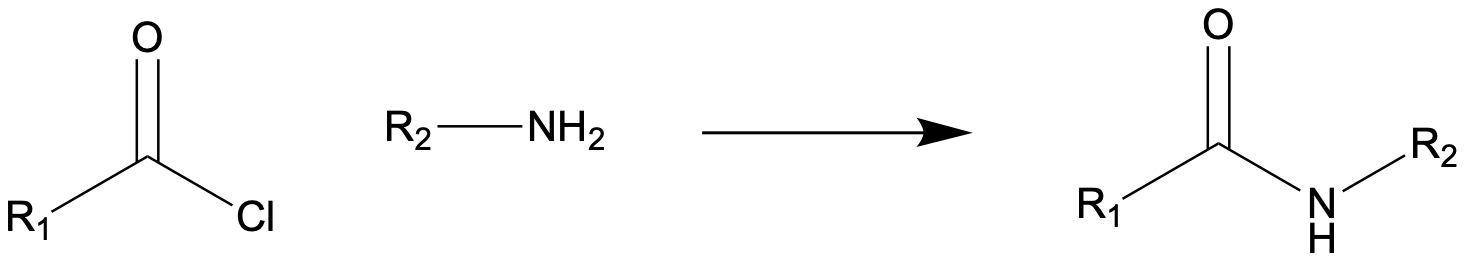
\includegraphics[width=0.75\textwidth]{Chapter2/Figs/Raster/rx_template.png}
% \caption[Reaction template]{An example of a reaction template for the synthesis of an amide}
% \label{fig:rx_template}
% \end{figure}
% These templates can be used for organic reaction prediction by building a catalogue of templates of as many organic reactions as possible. Then given some reactants and reagents as labelled graphs the problem of reaction prediction is transformed into one of subgraph searching to find the best matching general template in the catalogue. When that template is found it can be applied on the input to obtain the predicted outcome of the reaction. This approach was originally proposed and pioneered in the 1980s by E. J. Corey when he used templates for the reverse problem of retrosynthesis \cite{Corey1985Computer-assistedSynthesis}. The template-based approach had some success in forward reaction prediction for example as described in Ref~\cite{Klucznik2018EfficientLaboratory} a template-based model helped design synthetic pathways to a diverse set of 8 drug-like molecules. This method had considerably more success  in retrosynthesis though where there does not exist a single correct solution. One of the major limitation of template-based approaches when applied to forward prediction is scalability, meaning that the template library needs to be maintained and every time a new reaction is reported the associated template needs to be added to the template library. A further problem is that it is often not obvious which parts of the molecule are crucial for a given reaction. This means that given a reaction one can derive a smaller more general template or a larger one that is more specific for the particular reaction. This results in either too many templates matching a particular input resulting in many equally possible reaction outcomes or in the case of larger more specific templates the library will grow very big which results in very slow predictions.  \par

% \section{Data-driven reaction prediction}

% Modern approaches to reaction prediction increasingly rely on experimentally reported chemical reaction data instead of the knowledge of mechanisms. This can be advantageous for a number of reasons. The revolution of machine learning, pattern recognition and artificial intelligence resulted in a number of powerful methods developed in different fields such as natural language processing or graph generation that can be adapted for reaction prediction. These algorithms together with the several datasets containing hundreds of thousands or millions of reactions extracted from publications and patents using text mining have the potential for the development of successful models. These data driven models have the advantage that they can in principle build on all published reactions in the literature that no human chemist could look through to code up by hand. Furthermore, by learning from vast amount of data these machine learning models have the potential of learning complex chemical relationships resulting in better generalization. This is essential as the expectation for the reaction prediction models is to perform well on unseen molecules and potentially unseen reactions making them more than a simple searchable database. A limitation of these approaches is that the reaction databases often only contain the reactants and reagents and the major products, but not the minor products, yields, temperatures or other conditions. This makes the reaction prediction task an ill-posed problem. It is often the case that conditions such as temperature play a key role in determining the reaction outcome. For example in the case of enolate chemistry low temperature favours the formation of the kinetic, high temperature the thermodynamic enolate resulting in different selectivity \cite{Clayden2012}. Without specifying the temperature in these cases the major product cannot be determined. \par

% The first approach to data driven reaction prediction is very similar to the simple template based reaction prediction discussed above the only difference being that the templates are automatically extracted from the databases rather than being hand crafted \cite{Bgevig2015RoutePrediction, Kayala2012ReactionPredictor:Learning, Kayala2011LearningReactions,  Socorro2005ROBIA:Program}. This solves the issue of scalability but suffers from much of the same problems with the small templates being too general and large templates being too specific.  \par

% Machine learning models can also be used to directly predict the outcome of chemical reactions. These template-free approaches do not require any subgraph searching which results in much faster predictions. Another advantage is that since they are not directly memorizing templates from the training datasets they have the potential of better generalization by inferring some of the underlying reactivity trends. One of the first successful machine learning based model was proposed by Coley et. al. in 2017 \cite{Coley2017PredictionLearning}. Their approach builds on the template based models and combines them with neural networks. First a number of candidate products are generated using general templates extracted form the literature. These candidate templates are than scored using a neural network model trained to identify the major product. \par
% An improved model published by the same group has abandoned templates entirely \cite{ Coley2019AReactivity, Jin2017}. They have made use of the observation that usually only a small number of atoms and bonds participate directly in a chemical transformation. By considering the reactants and reagents as molecular graphs and the reaction as a series of graph edits they trained a reaction centre identifier network. This network selects a small number of atom pairs that are most likely to be involved in the reaction. All possible chemically valid graph edits are than considered on these centres. It is important to note that not all bond changes on the reaction centres have identical probabilities, and a product that results from more probable bond changes is itself more probable. This provides an initial ranking of the possible products. This generated ranking of products is then refined by a Weisfeiler-Lehman Difference Network, a type of graph convolutional neural network, to find the most probable product structure.  Together with the model they have also published a dataset of ca 480 000 reactions filtered from the text mining work of Lowe \cite{Lowe2012}. They have achieved 85\% accuracy on this dataset outperforming the previous state-of-the-art by more than 10\%. The key strength of this approach is that interpretability is built into the design of the algorithm. The way the model is predicting the sequence of graph edits is very similar to how humans would write arrow-pushing mechanisms of organic reactions\cite{Clayden2012}. This way one can get a direct insight into how the model is arriving at certain predictions. This is in contrast to previous reaction prediction approaches that were trying to directly learn mechanisms based on expert crafted rules as a supervised learning problem \cite{Bradshaw2019APaths, Kayala2012ReactionPredictor:Learning}.  \par

% In the 2010s natural language processing (NLP) and neural machine translation saw a huge revolution \cite{Young2018RecentProcessing}. This led scientists from different fields to the realization that many problems can be cast in a sequence-to-sequence formalism. This allowed them to use the powerful tools of NLP in a variety of applications. The first attempt to formulate the reaction prediction problem in a sequence-to-sequence manner came by Nam and Kim \cite{Nam2016LinkingReactions}. They have used a text based representation of organic molecules called SMILES \cite{Weininger1988, Weininger1989}. SMILES strings represent atoms with their chemical symbols and aromatic atoms with lowercase letters. Single and aromatic bonds are omitted while for double and triple bonds the specials characters \texttt{=} and \texttt{\#} are used. Branches are specified by enclosing them into parentheses. To encode cyclic structures a single bond in the ring is broken and the matching atoms are denoted by numbers. These rules lead to a large number of valid SMILES representations for larger molecules. To make the mapping injective a deterministic algorithm is used to enumerate the nodes of the molecular graph. Following this ordering a unique canonical text representation of organic molecules is obtained. This representation forms the basis for all of the text-based models discussed later. 
% A few examples of the SMILES syntax with the corresponding structures is shown below. 

% \begin{table}[h!]
% \begin{center}
%     \begin{tabular}{|c|c|}
%     \hline
%          SMILES & Structure \\
%          \hline
%          C & CH\textsubscript{4} \\
%          \lbrack Fe2+\rbrack & Fe\textsuperscript{2+} \\
%          C=O & CH\textsubscript{2}O \\
%          C\#N & HCN (cyan) \\
%          CCN(CC)CC & 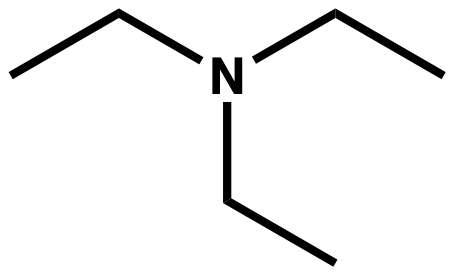
\includegraphics[width=0.75in]{triethyl_amine.png} \\
%          CC1=CC(CCC1)Br & 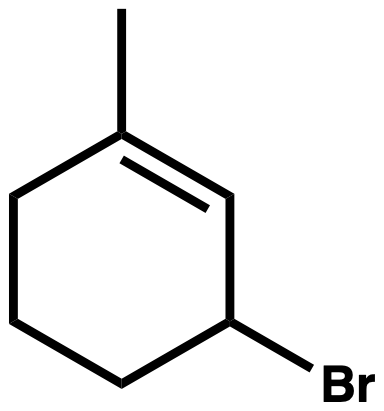
\includegraphics[width=0.7in]{cyclic.png} \\
%          \hline
%     \end{tabular}
%     \caption{Demonstration of the SMILES language}
%     \label{table:smiles}
% \end{center}
% \end{table}

% In the paper of Nam and Kim they formulated the reaction prediction problem as a translation task. The input SMILES corresponding to the reactant and reagent molecules are tokenized, so that each character of SMILES is equivalent to a word and the whole input is equivalent to a sentence. This sentence is than ``translated" by the model to the product SMILES. Neural machine translation models are trained using a large parallel corpus. This is available in the case of organic reactions from patents and publications or can be generated using templates of elementary reactions. The method of Nam and Kim served as an important proof of concept but could not match the accuracy of rule-based and graph-to-graph models. \par
% %The method was built on a neural network building block called gated recurrent unit (GRU) \cite{Cho2014LearningTranslation}. GRUs are a type of recurrent neural networks that process arbitrarily long inputs token by token, so that the hidden state representation of each token depends on the previous ones. %The model used in the paper is illustrated on Figure~\ref{fig:gru}. 
% %This model served as a proof-of-concept but could not match the accuracy of graph-to-graph and template based approaches. \par

% \iffalse
% \begin{figure}[htbp!] 
% \centering    
% \includegraphics[width=0.9\textwidth]{Chapter2/Figs/Raster/gru.png}
% \caption[GRU for reaction predictions]{The architecture used by Nam and Kim. The input SMILES string is tokenized into ``words", each token is embedded using a learnt embedding and processed by a three layer GRU network. The product is generated using attention mechanism.}
% \label{fig:gru}
% \end{figure}
% \fi

% The large breakthrough of sequence-to-sequence models for reaction prediction came after the introduction of a new and innovative architecture for neural machine translation by Vaswani et. al. \cite{Vaswani2017}. The so called Transformer model revolutionized the entire industry of machine translation and found use in many other areas of machine learning ever since. In the next section the Transformer architecture is described in detail followed by a discussion of the Molecular Transformer. 

% \section{The Molecular Transformer}

% \subsection{The Transformer architecture}

% The Transformer architecture was originally developed for machine translation tasks. It has an encoder-decoder structure. Both the encoder and the decoder are made up of so called transformer blocks that process the inputs by applying a multi-head scaled dot-product attention mechanism followed by layer normalization and some fully connected feed forward layers. In the following each part is described in detail. 

% \subsubsection{Encoder}
% The input to the model is a sentence made up of different words that are contained in a vocabulary. Each word in the vocabulary has a learnt fixed-length vector representation. Passing these vectors to the model would not be enough though as these vectors have no reference to where the given word appears inside the sequence. To encode this information as well another vector of the same length is added to each word-vector that depends on the position inside the sequence: \par

% \begin{equation}
%     PE_{(pos, 2i)}=\sin(pos/10000^{2i/d_{model}})
% \end{equation}
% \begin{equation}
%     PE_{(pos, 2i+1)}=\cos(pos/10000^{2i/d_{model}})
% \end{equation}

% This vector representation of the input text is passed into the transformer blocks. These consist of a multi-head attention layer with residual connection \cite{He2016DeepRecognition} followed by layer normalization \cite{Ba2016LayerNormalization} and a 2-layer fully connected feed forward neural network with ReLU activation. The encoder of the model is made up of $N=6$ transformer blocks as illustrated on Figure~\ref{fig:transformer}

% \begin{figure}[ht]
% \centering    
% \includegraphics[width=2.9in]{transformer_diagram.png}
% \caption{Graphical illustration of the full transformer model \cite{Vaswani2017}}
% \label{fig:transformer}
% \end{figure}

% \subsubsection{Multi-head scaled dot-product attention}
% The multi-head scaled dot-product attention is the heart of the Transformer model. It is a specific version of a general deep learning technique called attention. Given a set of vector \emph{values} and a vector \emph{query} the attention mechanism computes a weighted sum of the \emph{values} dependent on the \emph{query}. The sum represents a selective summary of the \emph{values} and the \emph{query} determines the importance of each vector, i. e. determines how much each \emph{value} vector is attended to.\par 
% The full attention mechanism operates by performing the following steps. Given some vector values $\bm{h_1}, \bm{h_2},\dots, \bm{h_N} \in \mathbb{R} ^{d_1}$ and a query $\bm{q} \in \mathbb{R} ^{d_2}$ \par

% \begin{enumerate}
%     \item First the attention scores $\bm{e} \in \mathbb{R}^N$ are computed. In the case of the scaled dot-product attention $d_1=d_2$ and $\bm{e}$ is simply defined as the scaled vector of projections $e_i=\frac{\bm{q}^\intercal \bm{h}_i}{\sqrt{d_1}}$
%     \item To generate the attention distribution $\bm{\alpha}$ the softmax of $\bm{e}$ is taken: 
%     \begin{equation}
%         \alpha_i=\frac{\exp{(e_i)}}{\sum_{j=1}^N \exp{(e_j)}} 
%         \label{eqn:softmax}
%     \end{equation}
%     \item Finally the attention distribution is used to take the weighted sum of the values to obtain the final output
%     \begin{equation}
%         \bm{a}=\sum_{i=1}^N \alpha_i \: \bm{h}_i \; \in \mathbb{R}^{d_1}
%     \end{equation}
% \end{enumerate}

% The scaling factor in the dot product serves the purpose of preventing some of the projection becoming overwhelmingly large which in turn would lead to the softmax function being sharply peaked around those values and being shallow everywhere else. This would result in very small gradients at most places that can substantially slow down the training.\par

% In the Transformer encoder the above described attention mechanism is used such that given a set of input vectors a new vector is calculated for all of them (being the query) from the others (being the keys). This is called self-attention. This way during training the model is able to learn which vectors (that are representing words or atoms) usually interact with each other. This interaction can result in a large value in the attention distribution. \par

% Usually the input, be it a chemical formula or a sentence contains a rich structure with the words affecting each others meanings in multiple ways. The problem with the simple self-attention mechanism is that by defining a single attention distribution for each input vector only one way of interaction can be learnt by the model. To give the model more flexibility to potentially learn more complex interaction structures multi-head attention was introduced. This mechanism maps the vectors to $h=8$ different lower dimensional spaces via a set of learnt linear transformations. The self-attention mechanism is than applied in these lower dimensional spaces simultaneously. The outputs of the different attention heads are finally concatenated and fed into a linear neural network layer. The whole mechanism is illustrated on Figure~\ref{fig:multihead_attention}

% \begin{figure}
% \centering    
% \includegraphics[width=2.2in]{mulithead_attention.png}
% \caption{Graphical illustration of the multi-head attention \cite{Vaswani2017}}
% \label{fig:multihead_attention}
% \end{figure}

% \subsubsection{Decoder}

% The outputs of the encoder which are $N$ vectors if the input sequence is $N$ words long are fed into the decoder which has a structure almost identical to the encoder. The first modifications concern the masking in the multi-head self-attention layers to make sure that every token in the output translation can only attend to the preceding ones. The second modification of the attention mechanism is making use of the encoder outputs by using them as keys whilst the queries are the outputs of the previous decoder layer. \par
% The generation of the translation happens in a sequential manner. First the embedding of the special \texttt{<start>} token is fed into the decoder and passed through the layers. The result is projected to a vector that has the same dimensionality as the size of the vocabulary. Finally the softmax function is applied to obtain the probability of the first word. The second word is generated by passing in the first word (and the \texttt{start} token) to the decoder, the third is generated by passing in the first and the second etc. This is called autoregressive translation. Finally the translation terminates either when the most probable next token is the special \texttt{<end>} token or when the maximum sequence length is reached. By multiplying together the next-token probabilities and normalizing with respect to the length of the output a confidence score of the translation can be obtained. 

% \subsection{Architecture of the Molecular Transformer}
% The Molecular Transformer architecture used throughout this work is based on the model described in Schwaller et. al. \cite{Schwaller2019MolecularPrediction}. The Transformer implementation used for this work is part of the OpenNMT natural language processing package \cite{Klein2017} which makes use of the PyTorch 1.2 framework \cite{Paszke2019PyTorch:Library}.\par
% Our implementation of the model uses a 256 dimensional learnt embedding for each SMILES token. The encoder and the decoder are both made up of 4 standard transformer layers and dropout is applied with probability 0.1 \cite{Srivastava2014Dropout:Overfittin}. For the optimization the Adam optimizer is used and the model is trained for 500 000 or 1 000 000 steps for the USPTO and Pistachio datasets respectively. Checkpoints are saved every 10 000 steps and the final model is obtained by averaging the weights of the last 20 checkpoints for USPTO and the last 10 checkpoints for Pistachio. \par
% \subsubsection{Datasets}
% The first dataset used in this work is the freely available USPTO dataset \cite{Lowe2012} that was filtered by Jin et. al. \cite{Jin2017}. Further filtering was preformed to remove some remaining duplicates or reactions that were erroneously text mined. These included examples such as reactions whose sole product is nitric acid, sulfuric acid, chloride ion etc. This way the final number of reactions in the dataset was 471 791 of which 377 419  were used for training, 23 589 for validation and 70 765 were used as a hold-out test set. The training set was augmented by an equal number of random equivalent SMILES strings. Augmentation can help the model to learn the underlying molecular graph from the SMILES sequence. \par
% The model trained in the way described above achieved 88.8\% Top-1 accuracy on the test set. This model was used throughout the interpretability experiments and is referred to as USPTO Transformer. \par
% The second dataset used was the commercial Pistachio dataset \cite{Mayfield2018Pistachio2.0}. This dataset contains over 9 million reactions text mined from US and EPO patents. This dataset was filtered similarly to USPTO to remove erroneous and duplicate reactions. It turned out that many of the 9 million reactions were duplicates corresponding to different patent IDs. In the end a dataset of 2 375 385 reactions was obtained of which 2 019 078 was used for training, 118 770 for validation and 237 537 for testing. \par
% The model trained as described above achieved 76.4\% Top-1 accuracy on the test set. Even though this looks like a substantially lower performance in reality the two models perform similarly well on new reactions. The possible reasons for the large difference in the measured performance on the held-out test sets are described in detail in Chapter~\ref{chap:interpr_molt}. This model obtained was also used in the interpretability experiments to test the effect of increased training set size on the models understanding of chemistry and is referred to as Pistachio Transformer in the rest of the thesis. \par

